To create an improved alignment and aesthetics of your TikZ figure with captions for six figures, you can use the `tikz` package along with `subcaption` to manage multiple subfigures within a single figure environment. Below is an example of how you can achieve this:

```latex
\documentclass{article}
\usepackage{tikz}
\usepackage{graphicx}
\usepackage{subcaption}

% Define colors for each type of deformation
\definecolor{unloaded}{RGB}{255,0,0} % Red
\definecolor{tension}{RGB}{0,128,0}  % Green
\definecolor{bending}{RGB}{0,0,255}  % Blue
\definecolor{shear}{RGB}{255,165,0}  % Orange

\begin{document}

\begin{figure}[h]
    \centering
    
    \begin{subfigure}[b]{0.45\textwidth}
        \centering
        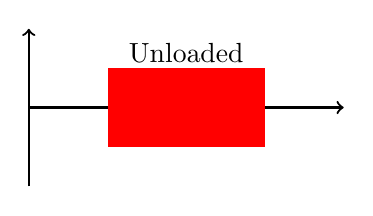
\begin{tikzpicture}
            \draw[thick,->] (0,0) -- (4,0);
            \draw[thick,->] (0,-1) -- (0,1);
            \fill[unloaded] (1,-0.5) rectangle (3,0.5);
            \node at (2,0.7) {Unloaded};
        \end{tikzpicture}
        \caption{Tension Strain}
        \label{fig:tension_strain}
    \end{subfigure}
    
    \hfill
    
    \begin{subfigure}[b]{0.45\textwidth}
        \centering
        \begin{tikzpicture}
            \draw[thick,->] (0,0) -- (4,0);
            \draw[thick,->] (0,-1) -- (0,1);
            \fill[tension] (1,-0.5) rectangle (3,0.5);
            \node at (2,0.7) {Tension};
        \end{tikzpicture}
        \caption{Bending Strain}
        \label{fig:bending_strain}
    \end{subfigure}
    
    \vspace*{\baselineskip}
    
    \begin{subfigure}[b]{0.4